% ------------------------------------------------------------------------
% Template zur Erstellung von Abschlussarbeiten an der Professur für
% Digitalisierung, E-Business und Operations Management
% Erstellerin: Jella Pfeiffer (Datum 08.10.2019)
% Überarbeitet von: Pascal Heßler, Paul Herbst
% zuletzt überarbeitet von: Pascal Heßler  am 15.06.2025
% ------------------------------------------------------------------------

% ------------------------------------------------------------------------
% Allgemeine Einstellungen
% ------------------------------------------------------------------------
\listfiles
\documentclass[
    12pt,
    paper=a4,
    headings=small,               % kleinere Überschriften
    twoside=false,                % einseitig, nur rechte Seiten
    listof=totoc,                 % Listen im Inhaltsverzeichnis aufnehmen
    bibliography=totoc,           % Literaturverzeichnis ins Inhltsvz. aufnehmen
    headsepline                   % Trennlinie unter Kopfzeile
    ]{article}

\usepackage[paper=a4paper,left=30mm,right=30mm,top=40mm,bottom=40mm]{geometry}
\usepackage[utf8]{inputenc}       % Damit können Umlaute ganz normal geschrieben werden.
\usepackage[english]{babel}     % Verwende deutsche, bzw. amerikanische Silbentrennung
%\usepackage[ngerman]{babel}       % Deutsche Alternative
\usepackage{scrlayer-scrpage}     % Paket für Kopf und Fußzeile. Kommentar: "scrpage2" veraltet in "scrlayer-scrpage" geändert
\pagestyle{scrheadings}           % Kopzeilenseitenstil
\usepackage{setspace}             % Zeilenabstand imlpementiert den Befehl 
% ------------------------------------------------------------------------
% Literatur
% ------------------------------------------------------------------------
% Achtung zur Einbindung der Literatur wird hier Biber verwendet und nich der Standard BibTex. In Sublime brauch man nichts verändern.
% 1. Sicherstellen, dass Biber installiert ist ->  in Tex Live vorinstalliert
% 2. Stellt eure Schreibumgebung um -> In TeXstudio: Optionen -> TeXstudio konfigurieren -> Erzeugen -> Standard Bibliographieprogramm
\usepackage[backend=biber,style=apa,natbib=false]{biblatex}
\DeclareLanguageMapping{american}{american-apa}         % Zitier Einstellung, bleibt auch im Deutschen!
\addbibresource{test.bib}       % Legt die Datei fest in der die Literatur liegt (z. B.: Export aus Citavi)
\usepackage{breakcites}                                 % Falls Zitationen nicht ans Zeilenende passen
\usepackage{csquotes}                                   % Erweitert die Möglichkeiten beim zitieren
% ------------------------------------------------------------------------
% Mathematische Symbole
% ------------------------------------------------------------------------
\usepackage{amssymb}
\usepackage{amsmath}        % Formattierung von Tabellen und Matritzen

% ------------------------------------------------------------------------
% Grafiken
% ------------------------------------------------------------------------
\usepackage{graphicx}       % Zum Einbinden von Grafiken
\usepackage{subfigure}      % Um Bilder innerhalb einer Figure anzuordnen (Bild a b c d...)

% ------------------------------------------------------------------------
% Tabellen
% Um einfache Tabellen zu erstellen kann https://www.tablesgenerator.com/ verwendet werden.
% ------------------------------------------------------------------------
\usepackage{tabularx}       % Ermöglicht weitere Tabellen Einstellungen
\usepackage{multirow}       % Ermöglicht Zellen zu verbinden
\usepackage{booktabs}       % Tabellen Midline Topline etc.
\usepackage{float}          % Tabelen Positionierung
\usepackage{longtable}      % Ermöglicht Tabellen über mehrere Seiten hinweg, so dass sie noch dasselbe Format besitzten ftp://ftp.fu-berlin.de/tex/CTAN/macros/latex/required/tools/longtable.pdf

% ------------------------------------------------------------------------
% Abkürzungen und Glossar
% VERWENDUNG: Hier die Abkürzungen definieren und im Text verwenden mit \gls{AI} oder \glspl{AI} für Plural
% Zur Aktualisierung "makeglossaries" bzw. "makeglossaries master" ausführen und dann nochmal kompilieren
% ------------------------------------------------------------------------
\usepackage[acronym,toc,nonumberlist]{glossaries} % Ermöglicht die Verwendung von Abkürzungen und Glossar

\makeglossaries

\newacronym{ai}{AI}{Artificial Intelligence}        % Hier werden die Abkürzungen definiert
\newacronym{ml}{ML}{Machine Learning}
\newacronym{nlp}{NLP}{Natural Language Processing}
\newacronym{ca}{CA}{Combinatorial Auctions}

% **********************************************************************************************************************
% Folgende Pakete sind rein optional und etwas komplexer in ihrer Umsetzung nur für etwas erfahrenere LaTeX User
% **********************************************************************************************************************
% \usepackage{siunitx}      % Ausrichten von Tabellen an dezimalstellen (Umsetzung etwas komplizierter)
% \usepackage{rccol}        % Ein Neues Format R (wird wahrscheinlich mit dem Folgenden R zu Problemen führen) und sorgt, dass nach , ausgerichtet wird und automatisches runden in Tabellen wird ermöglicht
% \usepackage{fltpoint}     % Gehört zu rccol
% \usepackage{dcolumn}      % Gehört zu rccol
%
% \newcolumntype{L}[1]{>{\raggedright\arraybackslash}p{#1}}       % Linksbündig mit Breitenangabe
% \newcolumntype{C}[1]{>{\centering\arraybackslash}p{#1}}         % Zentriert mit Breitenangabe
% \newcolumntype{R}[1]{>{\raggedleft\arraybackslash}p{#1}}        % Rechtsbündig mit Breitenangabe
% \newcolumntype{x}[1]{!{\centering\arraybackslash\vrule width #1}}


% ------------------------------------------------------------------------
% Lua Wordcount
% ------------------------------------------------------------------------
\usepackage{luacode}
% loads lua script
\directlua{dofile(kpse.find_file"word_count.lua")}
% defining latex commands to use lua functions easier 
\def\setwordthreshold#1{
  \directlua{packagedata.word_count.set_threshold(\number#1)}%
}

\def\startwordcount{
  \directlua{
    luatexbase.add_to_callback(
    "pre_linebreak_filter",
    packagedata.word_count.callback,
    "word_count"
    )
  }
}

\def\stopwordcount{
  \endgraf %% force paragraph
  \directlua{
    luatexbase.remove_from_callback(
    "pre_linebreak_filter",
    "word_count"
    )
  }
}

% Creates Logfile
\def\dumpwordcount{%
  \directlua{packagedata.word_count.dump_total_word_count()}
}
% This returns the normalized sides at the current position
\def\dumprelativwordcount{%
  \directlua{packagedata.word_count.dump_relativ_word_count()}%
}

% This returns the word count at the current position.
\def\currentwordcount{%
  \directlua{packagedata.word_count.current_word_count()}
}

% Text result
\def\prettyresult{\directlua{packagedata.word_count.pretty_result()}}

% ------------------------------------------------------------------------
% Sonstige
% ------------------------------------------------------------------------
\usepackage{scrhack}        % Löst unnötige Warnungen!
\usepackage{color}          % Ermöglicht Text einzufärben \pagecolor{FARBE}  \color{FARBE} \textcolor{FARBE}{TEXT} \colorbox{FARBE}{TEXT}
\usepackage{hyperref}       % Ermöglicht URLS schreibweise ist z.B. \url{http://www.uni-giessen.de}

\usepackage{eurosym}        % Für Euro Symbol \euro{} oder \eruo (Unterschieden sich bezüglich Leerzeichen danach)

\usepackage{framed}         % Einrahmen von Texten mit der shaded-Umgebung.

\usepackage{pdflscape}      % Querformat möglich über \begin{landscape} \end{landscape}
\usepackage{tikz}           % need for tikzpicture



% ------------------------------------------------------------------------
% Fein Justierungen
% ------------------------------------------------------------------------
\DeclareMathOperator*{\argmax}{arg\,max}

\renewcommand{\floatpagefraction}{.9}     % vorher: .5

\newenvironment{packed_enum}{
\begin{enumerate}
  \setlength{\itemsep}{1pt}
  \setlength{\parskip}{0pt}
  \setlength{\parsep}{0pt}
}{\end{enumerate}}

%\setlength{\parindent}{0pt}                    % Kein Einzug beim Absatzbegin
\setlength{\parskip}{1pt plus 0pt minus 1pt}    % Abstand zwischen 2 Absätzen

% Kapitel Überschriften in Schriftart mit Serifen
%\setkomafont{sectioning}{\normalfont\normalcolor\bfseries}
% Gestaltung der Kopfzeilen
\ohead{\pagemark} \cfoot{} \cohead{} \ihead{\headmark}
\setkomafont{pagehead}{\normalfont\bfseries}
%\setkomafont{pagenumber}{\normalfont\bfseries} \automark{section}

%% ---------------------------------
%% | Information about the thesis  |
%% ---------------------------------

\newcommand{\mytype}{Seminar / Master / Bachelor Thesis}

\newcommand{\myname}{Your Name}
\newcommand{\matricle}{matriculation number}
\newcommand{\mytitleen}{Title of the Thesis in English }
\newcommand{\mytitlede}{Title of the Thesis in German }

\newcommand{\myinstitute}{At the Department of Economics and Management \\ Institute for Information Systems (WIN) \\  Information Systems III   }

\newcommand{\reviewerone}{Prof. Dr. Jella Pfeiffer}
\newcommand{\supervisor}{Vorname Nachname}
\newcommand{\submissiontime}{Date of Submission}

%% -------------------------------
%% |  Information for PDF file   |
%% -------------------------------
%% IM: Auto-Fill this information
\hypersetup{
 pdfauthor={\myname},
 pdftitle={\mytitleen},
 pdfsubject={\mytype},
 pdfkeywords={\mytype}
}


\hypersetup{hidelinks}                 % Versteckt die Links im PDF (optisch)
% ----- ende der präambel ----------------------------------
% Start des Dokuments
% ----------------------------------------------------------
\begin{document} 
\pagenumbering{Alph}                  % Löst unnötigen Warnungen
%% titlepage.tex
%%

% coordinates for the bg shape on the titlepage
\newcommand{\diameter}{20}
\newcommand{\xone}{-15} % start left
\newcommand{\xtwo}{150} % ende right
\newcommand{\yone}{20} % start top
\newcommand{\ytwo}{-230} % end bottom

\begin{titlepage}
    \begin{onehalfspace}

% bg shape
        \begin{tikzpicture}[overlay]
            \draw[color=gray]
            (\xone mm, \yone mm)
            -- (\xtwo mm, \yone mm)
            arc (90:0:\diameter pt)
            -- (\xtwo mm + \diameter pt , \ytwo mm)
            -- (\xone mm + \diameter pt , \ytwo mm)
            arc (270:180:\diameter pt)
            -- (\xone mm, \yone mm);
        \end{tikzpicture}

        \vspace{-1cm}
        
\includegraphics[width = 0.25\linewidth]{graphics/KITLogo.jpeg}%
        \hfill
        
\includegraphics[width =  0.25\linewidth ]{graphics/win_logo_en}
        \vspace*{0.5cm}
       \hrule
        \vspace*{1cm}
        \begin{center}
            \Huge{\mytitleen} \\
            \Huge{---}\\
            \Huge{\mytitlede} \\ 
            \vspace{1cm}
            \normalsize{ \mytype\\ of \\}

            \vspace*{1cm}
            \large{\myname}\\
            \large{\submissiontime}\\
            \large{\matricle}\\
            \vspace*{2cm}
            \large{  \myinstitute}

        \end{center}
        \vspace*{1cm}
        \normalsize{
            \begin{center}
                \begin{tabular}[ht]{l c l}
                    Reviewer: & \hfill & \reviewerone \\\
                    Advisor:  & \hfill & \supervisor  \\
                \end{tabular}
            \end{center}
        }


    \end{onehalfspace}
\end{titlepage}
              % Titelseite einbinden


\pagenumbering{Roman}                 % Löst unnötigen Warnungen
\setcounter{page}{2}                  % setzt die Seitenzahl auf 2
% ------------------------------------------------------------------------
% Verzeichnisse
% ------------------------------------------------------------------------
\tableofcontents                                                % Inhaltsverzeichnis einbinden
\newpage
\printglossary[type=\acronymtype]  % Abkürzungsverzeichnis einbinden
\newpage


% settings for word counting
\setwordthreshold{2}                   % min chars in a row to count as word
\startwordcount                        % start counting words

% ------------------------------------------------------------------------
% Hauptarbeit (hier werden alle Kapitel eingebunden)
% ------------------------------------------------------------------------
\pagenumbering{arabic}                  % Löst unnötige Warnungen
\setstretch{1.5}

%!TEX root = ../master.tex


\section{Introduction} \label{chap:introduction}
Scientific papers have standardized structures. There are different standards for different types of papers. You should make sure that the paragraphs are not too short (i.e., at least 3-4 sentences). This is still a rather short paragraph.

\noident This would then be a new paragraph. But this paragraph would be too short.


\section{Brief Overview of the Content of Chapters}
Below we give you a few tips for writing the different chapters.


\subsection{Introduction}
\begin{enumerate}
    \item Problem definition and motivation
    \item State of research, building on this, identify research gap and research question(s)
    \item Aim of the work and own methodological approach to answering the research question(s): Paragraph usually begins with: The goal of this thesis/work/manuscript is ...
    \item Expected scientific (and practical) contribution [=Contribution]
    \item Sometimes follows: Outline [formulated]
\end{enumerate}


\subsection{Chapter on Related Work/Theories/Literature}
\begin{enumerate}
    \item What theories and principles are there?
    \item Focus on a few, central ones
    \item Absolute basics do not need to be explained. You can assume that the readers already know a lot. (specialist audience!)
    \item Often subdivided into subheadings according to the different types of foundations/theories
    \item Not yet refer to own work and own approach, so never "pre-reference"
\end{enumerate}

The aim is to make the research gap clear. You are also welcome to explicitly name and elaborate on this. [This is the only place where implicit reference is made to your own work.]

The other chapters between the basic chapters and the conclusion are individually very different. Your own contribution should be in the foreground in these further chapters.


\subsection{Discussion}
\begin{enumerate}
    \item The discussion reflects the results of the work
    \begin{enumerate}
        \item In empirical works, the results section reports the data situation (e.g., hypothesis tests) in a very dry manner and these results are only interpreted in the discussion.
        \item In purely normative papers, the discussion often coincides with the presentation of the results, as the two parts are more difficult to separate.
    \end{enumerate}
\end{enumerate}


\subsection{Conclusion}
Depending on the length of the thesis, this chapter does not need to be subdivided.
\begin{enumerate}
    \item Summary
    \begin{enumerate}
        \item Varies depending on the level of detail of the previous discussion. In empirical papers: Brief summary of findings and higher-level analysis of results
        \item Reference to research questions and the extent to which they have been answered
    \end{enumerate}
    \item Limitations/critical appraisal and outlook
    \begin{enumerate}
        \item What problems were encountered in the present work?
        \item How can these be addressed in future work?
        \item What other future, related research topics should be addressed in the future?
    \end{enumerate}
    \item Contribution:
    \begin{enumerate}
        \item What conclusions can be drawn?
        \item What contributions does the work make to research and practice? [Contribution]
    \end{enumerate}
\end{enumerate}






%!TEX root = ../master.tex

\subsection{Die Erstellung und Verwendung von Abkürzungen} \label{chap:abbreviations}
Dieses Kapitel demonstriert die Verwendung des \emph{glossaries} packages zur automatischen Verwaltung von Abkürzungen. Abkürzungen werden in der Präambel in der Datei \emph{master.tex} definiert.

\gls{ai} is a broad field focusing on the creation of smart machines. The growth of \gls{ai} and \gls{ml} has led to significant advancements in \gls{nlp}.

\gls{ai} is a broad field focusing on the creation of smart machines. The growth of \glspl{ai} and \gls{ml} has led to significant advancements in \gls{nlp}.


Wichtig: damit die Abkürzungen korrekt im Abkürzungsverzeichnis erscheinen, muss der Befehl \emph{makeglossaries} bzw. \emph{makeglossaries master} in der Konsole ausgeführt werden. Anschließend muss das Dokument neu kompiliert werden.

%!TEX root = ../master.tex

\section{Figures and Tables}
Here you will find examples of how to insert figures and tables.


\subsection{Experimental Design}

In the NO-FILTER condition, ten randomly chosen projects were shown to the participant on the overview page
(see Figure \ref{fig:overview}). There was a short description of each project on the list,
as well as a photo, the name, the amount of money already lent to the project
and one sentence describing the project. The participants could then click on
each project in any order to access the detailed project description page,
which described the project in a longer text of mostly two to three paragraphs (see Figure \ref{fig:procedure1}).
In addition, information was provided on the repayment schedule. The participants could navigate
between the overview page and the detailed description in any order and as long they wanted.
Finally, they had to choose one project by clicking on the “Choose” button in the detailed project description.\\
Condition STANDARD: Filter Followed by Joint Evaluation\\
In the STANDARD condition, participants could set filters for several criteria (see Figure \ref{fig:firststep}).
They were not forced to set filters, but all participants used them.
Subsequently, they were asked to rank the order of the filter criteria they selected according to their importance (see Figure \ref{fig:secondstep}).
Afterwards, they saw the same overview page and the detailed project description page as the participants in the NO-FILTER condition (see Figure \ref{fig:overview} (right) and Figure \ref{fig:procedure1}).
However, the ten projects they saw were not randomly chosen, but selected on the basis of their filters and importance sorting.\\
\begin{figure}[h]
    \centering
    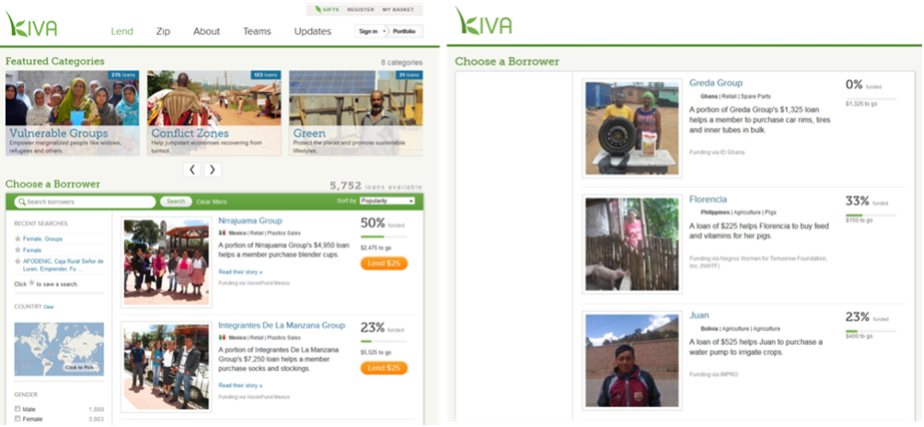
\includegraphics[width=0.8\textwidth]{graphics/Bild1}
    \caption{Overview page. Left: Original Screenshot from KIVA. Right: Screen that participants saw in the experiment (Overview Page).}
    \label{fig:overview}
\end{figure}

\begin{figure}[h]
    \centering
    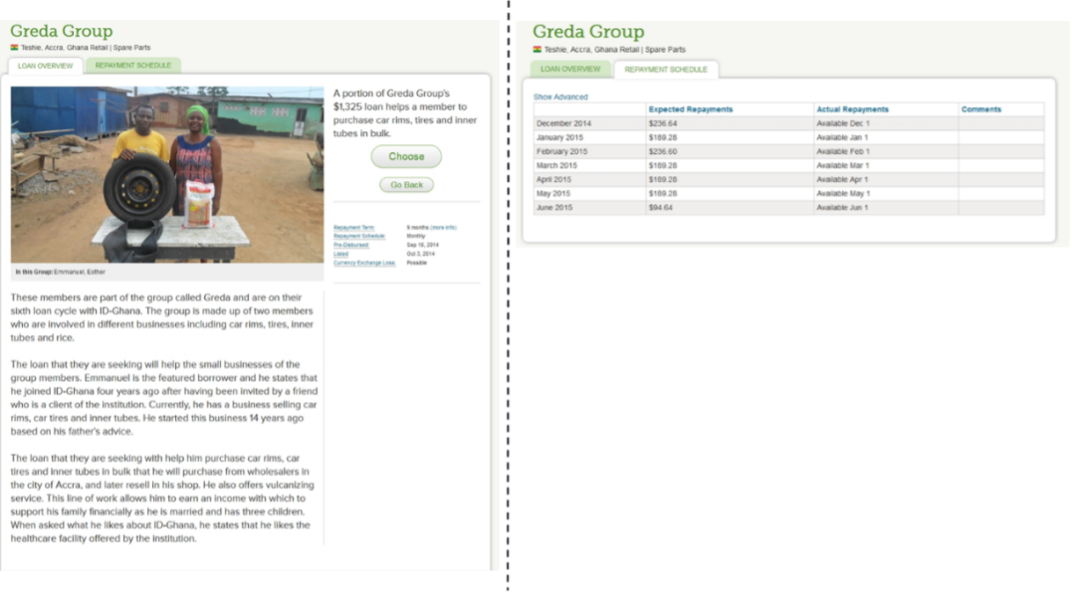
\includegraphics[width=0.8\textwidth]{graphics/Bild2}
    \caption{ Detailed Project Description Page with repayment schedule.}
    \label{fig:procedure1}
\end{figure}
As filter
criteria, the participants could set: country, gender, sector, groups or
individuals, and attributes (for example, green, start-up, youth, fair trade,
etc.). These are the same filters the KIVA offered on the standard screen at
the time of our experiment. If less than ten projects met the filter criteria,
the least importance criteria were relaxed. For example, if a participant had
set the two filters gender=females and sector=education and had indicated
sector as more important than gender, but only eight projects fulfilled both
criteria, we selected these eight projects and then selected another two
projects randomly drawn from all projects in the education sector with
entrepreneurs of any gender. Participants were fully informed about this procedure
(see text in Figure \ref{fig:secondstep}).\\
\begin{figure}[h]
    \centering
    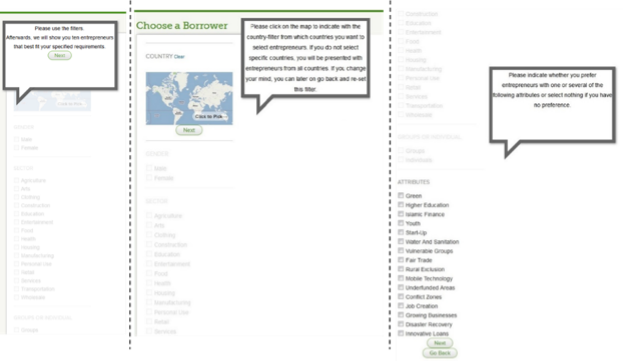
\includegraphics[width=0.8\textwidth]{graphics/Bild3.png}
    \caption{ Detailed Project Description Page with repayment schedule.}
    \label{fig:firststep}
\end{figure}

\begin{figure}[h]
    \centering
    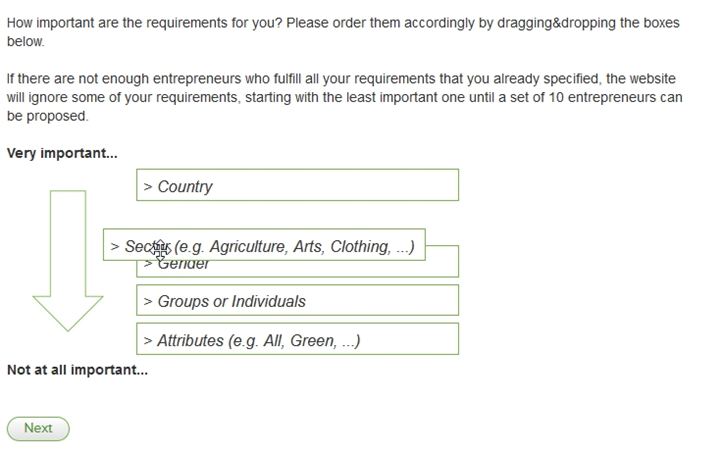
\includegraphics[width=0.8\textwidth]{graphics/Bild4.png}
    \caption{ Detailed Project Description Page with repayment schedule.}
    \label{fig:secondstep}
\end{figure}


\subsection{Procedure}
Figure \ref{fig:procedure2} illustrates the experimental
procedure. In addition to a lab session that lasted about 45 minutes, the
participants completed two short online surveys: a pre-questionnaire two weeks
before this session and a post questionnaire 12 weeks later. In the pre-questionnaire,
we asked participants what their goals would be when lending money, the
situation-specific thinking style they would use when deciding this, and other
control variables, like their age and gender. The two-week delay allowed us to
measure the constructs without making them overly salient during the lab study,
thereby reducing the risk that the elicitation of these constructs would
potentially influence participants during the lab session. In the post
questionnaire, we asked the participants how satisfied they still were with
their choice in the lab, and how often they had revisited the platform since
that time. We considered the 12-week delay between the lab session and the post
questionnaire sufficiently long to gauge the impact of our manipulations and of
any long-lasting effects resulting from the experience in the experiment. There
was no attrition between the pre-questionnaire and main experiment (the
pre-questionnaire was a pre-requisite in register for the experimental
session), but only 69 (78.4\%) of the 88 participants completed the post
questionnaire.\\
\begin{figure}[h]
    \centering
    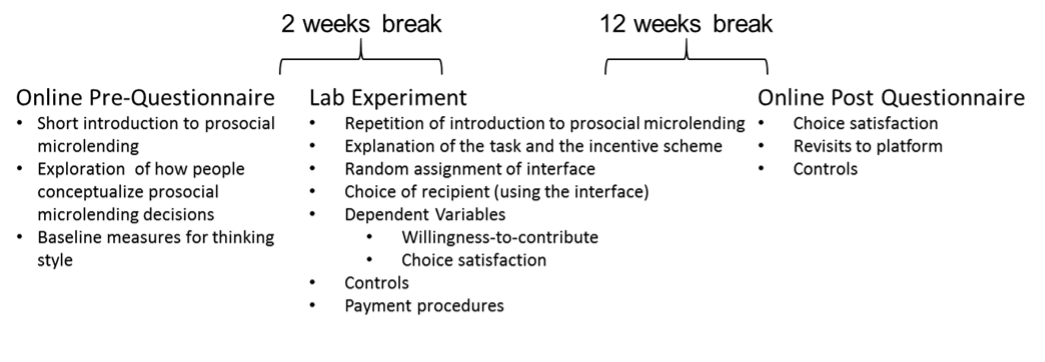
\includegraphics[width=0.8\textwidth]{graphics/Bild5}
    \caption{ Detailed Project Description Page with repayment schedule.}
    \label{fig:procedure2}
\end{figure}
\subsection{Results}
\bold{ Testing our Hypotheses}
Table \ref{tab:descriptive} shows
the descriptive statistics of the dependent variables and mediators that we use
for testing our hypotheses. In particular, we conceptualize analyticalStyle
(experientialStyle) as the change in analytical (experiential) thinking style
evoked by the interface in the main experiment. In particular, we calculate the
difference between the scores of the analytical (experiential) thinking style
scales of the pre-questionnaire and the main questionnaire. We see that, after
a choice has been made, the thinking style becomes less analytical (two-sided
t-test, $ t(87)=4.46, p<0.01 $ ) and slightly more experiential ($t(87)=-1.74,
p=0.09$). (A positive value indicates an increase in the analytical/experiential
thinking style after the participants had made their choice in the lab
experiment, compared to the one they had anticipated in the pre-questionnaire.)
Furthermore, Table \ref{tab:descriptive}
reveals that the perceived strategy restrictiveness is, with an average of
3.60, rather in the middle of the scale. In contrast, immediately after the
participants had made their choice, their choice satisfaction is relatively
high at 5.45, and also remains on a high level when asked again 12 weeks later
in the post questionnaire (both scales range from 1 to 7). Finally, the
participants were rather generous: On average, they contributed 60.81 to the
chosen project and only took 39.19 in cash.\\
\begin{table}[h]
    \centering
    \renewcommand{\arraystretch}{1.2} % Adjust row height for better readability

    \begin{tabular}{p{5cm} p{0.8cm} p{0.8cm} p{5cm} p{0.8cm} p{0.8cm}}
        \toprule
        \textbf{Variable} & \textbf{Mean} & \textbf{SD} & \textbf{Variable} & \textbf{Mean} & \textbf{SD} \\
        \midrule
        \multicolumn{6}{l}{\small{\textit{Dep var. variables and mediators (thinking style: [1,5], all others [1,7])}}} \\
        Analytical Style & -0.37 & 0.79 & Experiential Style & 0.12 & 0.65 \\
        Perceived Strategy Restrictiveness & 3.60 & 1.26 & Choice Satisfaction (Main Questionnaire) & 5.45 & 1.08 \\
        Choice Satisfaction (Post Questionnaire) & 5.00 & 1.27 & Willingness-to-Contribute & 60.81 & 25.11 \\
        \bottomrule
    \end{tabular}
        \caption{Descriptive statistics of mediators and dependent variables }
    \label{tab:descriptive}
\end{table}
To test our Hypotheses 1, 2, and 3 about the effects of the interfaces on the
different dimensions of the platform’s success, we conducted a separate OLS
regression for choice satisfaction and willingness-to-contribute. We computed
two models for choice satisfaction, one that regresses on the choice
satisfaction that was reported immediately after the choice in the lab (choice
satisfaction main) and one that regresses on the choice satisfaction reported
in the post questionnaire (choice satisfaction post). The STANDARD condition
was coded as the reference, so that the coefficients for NO-FILTER and SINGLE
reflect the respective differences when comparing these conditions with
STANDARD. In particular, the difference between the condition that supports an
attribute-based selection and the one that does not, is reflected in the
coefficient for NO-FILTER. The difference between the condition that supports
joint evaluation and the one that supports only single evaluation is reflected
in the coefficient for SINGLE. Table \ref{tab:hypothesis_results}
summarizes the results of the three models. … \\
\begin{table}[h]
    \centering
    \begin{tabular}{l c c c c c c}
        \hline
        & \multicolumn{2}{c}{Choice Sat. Main} & \multicolumn{2}{c}{Choice Sat. Post} & \multicolumn{2}{c}{WtC} \\
        Reference Category:\\ STANDARD & Coeff. & p-value & Coeff. & p-value & Coeff. & p-value \\
        \hline
        NO-FILTER & .039 & 0.887 & .131 & 0.727 & -3.42 & 0.603 \\
        SINGLE & -.618 & 0.029 & -.429 & 0.266 & 12 & 0.073 \\
        Constant & 5.60 & <0.010 & 5.10 & <0.010 & 57.92 & <0.010 \\
        N & 88 &  & 69 &  & 85 &  \\
        \hline
    \end{tabular}
    \caption{Results of Hypothesis 1, Hypothesis 2, and Hypothesis 3.}
    \label{tab:hypothesis_results}
\end{table}
\textbf{\textit{Additional Analyses}}

AND SO ON





%!TEX root = ../master.tex
\section{Citation}

\subsection{Citing Literature}
We recommend using reference management programs like Zotero, Citavi, or Mendeley:
\begin{itemize}
    \item Manage PDF documents
    \item Automatic import of source information via plug-ins in the browser, PDF, databases, etc.
    \item Annotations, notes, tagging, ...
    \item Comparison of the software: \url{https://mediatum.ub.tum.de/doc/1316333/1316333.pdf}
    \item These programs cannot do magic; check if the stored information is correct! This is your responsibility!
    \item Garbage in \( \rightarrow \) Garbage out
\end{itemize}

\subsection{Citation Style}
\begin{itemize}
    \item American Psychological Association (APA) \( \geq \) 6 Citation style
    \item Please view very good instructions online: \url{https://www.scribbr.de/category/apa-standard/}
    \item Both direct quotations (adopted passages in the wording) and indirect quotations (adoption of an idea) must be identified.
    \item Each source used in the paper (book, article in a collective work, journal article, website (with retrieval date)) must be referenced!
    \item In most cases, there is a publication behind a website, e.g.: behind \url{https://sloanreview.mit.edu/projects/artificial-intelligence-in-business-gets-real/} hides the following source: \textcite{ransbotham2018}.
\end{itemize}

\subsection{Indirect Citation (In-text citation)}
Parenthetical: There is a correlation between social media usage and anxiety symptoms in teenagers \parencite{barr1999}.

Narrative: \textcite{barr1999} found a correlation between social media usage and anxiety symptoms in teenagers.

\textbf{One Author:}
\begin{itemize}
    \item An early study of this phenomenon\parencite{barr1999}...
    \item \textcite{barr1999} already dealt with this phenomenon...
    \item  Already in 1999 Barr dealt with this special phenomenon...

\end{itemize}

\textbf{Two Authors:}
\begin{itemize}
    \item \parencite{cadogan2013}
    \item But: Already \textcite{cadogan2013} dealt with this special phenomenon.
\end{itemize}

\textbf{Three or More Authors:}
\begin{itemize}
    \item generally only ever cite the first author and then with et al.
    \item Example: \parencite{beutel2004}.
\end{itemize}

\textbf{Using multiple sources:}
\begin{itemize}
    \item The various sources are separated by a semicolon and sorted alphabetically
    \item Example: \parencite{barr1999, cadogan2013, smith2015, smith2017}.
\end{itemize}

If you cannot find the original source, you should cite it through the secondary source using “as cited in”: \parencite[as cited in Parker, 2021]{smith2017}.

\subsection{Direct Quotes}

\begin{enumerate}
    \item Literal quotations must be reproduced verbatim and placed between quotation marks!
    \item Example: APA direct quote According to a recent paper, “quotes can be useful in academic writing” \parencite[p. 25]{singh2019}.
    \item Three If the quote is 40 words or more, format it as a block quote: \begin{quote}
        Lawmakers and regulators must stop pharmaceutical companies from marketing drugs such as OxyContin and establish stronger guidelines on how and when doctors can prescribe them. These drugs are often the last resort for people with cancer and other terminal conditions who experience intense pain. But they pose a great risk when used to treat the kinds of pain for which there are numerous non-addictive therapies available. \parencite{editorialboard2018}.
    \end{quote}
    \item  If you only want to quote an excerpt directly, you can use [...] to indicate that you have left something out. It is
important to note that this does not change the content of the quoted text.
    
    '[...] it is possible that participants fewer attended effectiveness ratings for charities because they wanted to have agency when making charitable
decisions [...' \parencite[p. 827]{ransbotham2018}.

\end{enumerate}

%!TEX root = ../master.tex


\section{Bibliography}


\subsection{Basics}
List all materials used. Sort alphabetically by the author's name (within an author, chronologically, with the oldest source first). Use indents. Do not sort by source type. Do not use bullet points.


\subsection{DOI or URL}
Works that can be accessed online usually have a URL or DOI (digital object identifier). A DOI is often used for scientific publications and books, while a URL is more common for other online publications.

Use the following guidelines:
\begin{itemize}
    \item If available, always add a DOI.
    \item A DOI is preferred over a URL (because it never changes).
    \item Include the protocol (\texttt{http://} or \texttt{https://}) for both DOIs and URLs.
    \item Do not add a period after the DOI or URL.
\end{itemize}
\subsection{Different type of Sources}
\begin{Large}
    See Word template for different examples
\end{Large}
%!TEX root = ../master.tex
\section{Combinatorial Auctions}
\label{chap:combinatorialAuctions}

This is an excerpt from a sample chapter.

\emph{Combinatorial auctions} (CAs) are a part of electronic
market design. Research in electronic market design joins two
disciplines: economics and computer science. Economical research
focuses on game theoretical aspects by analyzing strategic
behavior of self-interested agents. From the viewpoint of computer
science, computational problems are addressed, such as finding the
optimal allocation in auctions. As this work concentrates on
computational aspects, we assume that the reader has a stronger
background in computer science than in economics. Thus, in this
chapter we will point out the main ideas of the economical
perspective to provide some basic knowledge in this area.

\subsection{Mechanism Design}
\subsubsection{Definition}
Mechanism design was introduced by \textcite{Knapp.2011}. It
aims at implementing system-wide solutions to problems in
non-cooperative environments with multiple self-interested agents.
Such problems can be political elections, public projects in which
the participants themselves have to invest money, or allocation
problems. Given that agents hold only private information about
their preferences, a structure has to be chosen in which in
equilibrium each agent behaves according to the designer's or principal's
intentions. The designer can either act on behalf of the society, for
example when collecting taxes for a public project, or she can
pursue self-interests when, for instance, being an auctioneer.

Since the agents' information is private, the principal faces the
problem that the agents might lie about their real valuations in
order to influence the outcome according to their preferences. In
most cases, whenever such manipulations occur, they damage the
resulting system-wide welfare \parencite{Grant.2011}. Thus, simply asking
the participants to reveal their preferences is unfavorable.
Therefore, the principal has to define other rules which lead to
the desired outcome. The most common solution to this problem is
to introduce monetary transfers providing incentives for the
agents to behave truthfully.

In mechanism design two economic areas are joined: \emph{game
theory} and \emph{social choice theory}. In game theory the
agents' strategies are analyzed, and in social choice theory an
outcome is selected according to a set of agents' preferences. The
outcome in social choice theory is determined by a social choice
function, which is to be implemented by a mechanism. Formally we
have a set of possible outcomes $O$ and agents $i \in I$, $|I|=n$.
Each agent $i$ has a type $\theta_i \in \Theta_i$ reflecting the
possible preference sequences the agent can have. The type captures
all of the agent's private information relevant to her decision.
The agent's utility $u_i(o,\theta_i)$ over each outcome depends on
her type; while $u_i(o_1,\theta_i)>u_i(o_2,\theta_i)$ means that
the outcome $o_1$ is preferred over the outcome $o_2$. The social
choice function maps from the space of all types $\Theta$ to the
space of all outcomes $O$,
\begin{eqnarray}
% \nonumber to remove numbering (before each equation)
  f:\Theta_1 \times\Theta_2\times...\times\Theta_n\rightarrow O.
\end{eqnarray}
Examples for such social choice functions are allocation problems or political voting
protocols in which a candidate or a party is chosen. The most common objective of a social choice function is
the maximization of the social welfare, the so called
\emph{allocative-efficiency} \parencite{Bastian.2011}. It maximizes the sum of
all utilities over all agents:
\begin{eqnarray}
\label{Efficient}
% \nonumber to remove numbering (before each equation)
  f(\theta)=\argmax_{o \in O} \sum_{i \in I} u_i(o,\theta_i).
\end{eqnarray}
Another objective is \emph{individual rationality}; the agent's
payoff is never less when participating in the mechanism than her
payoff without participating. Additionally there is \emph{Pareto
optimality}. An outcome is Pareto optimal whenever none of the
agents could perform better without causing another agent to
perform worse than in the current situation.

So far, we have learned what a social choice function is, and what
typical objectives for the choices of outcomes are. Now, a
mechanism has to be found which implements a given social choice
function with one or several of these objectives. For this
purpose, the agents' possible strategies have to be specified
together with an outcome function based on these strategies. The
mechanism should guarantee an implementation despite the
self-interest of the agents \parencite{Bastian.2011}. Mathematically, a
mechanism $M$ is defined on the strategy spaces $S_i$ of the
agents:
\begin{equation}\label{MechanismDefinition}
  M=((S_1,...S_n),g(\cdot))\\
  g:S_1\times...\times S_n\rightarrow O,
\end{equation}
where $g$ is an outcome function and $S_i$ denotes all strategies
or actions an agent $i$ is allowed to take. A mechanism implements
a social choice function if there is an equilibrium strategy
profile $s^\ast(\cdot)=(s^\ast_1(\cdot),...,s^\ast_n(\cdot))$ of
the game induced by $M$ so that
\begin{equation}\label{MechanismImplements}
    g(s^\ast_1(\theta_1),...,s^\ast_n(\theta_n))=f(\theta_1,...,\theta_n),
      \quad \forall
      (\theta_1,...,\theta_n)\in(\Theta_1,...,\Theta_n),
\end{equation}
where $s^\ast_i(\theta_i)$ is the strategy agent $i$ with type
$\theta_i$ plays in the equilibrium. Please note that the
equilibrium concept is not specified in this definition. It could,
for example, be a Nash equilibrium. In this case, given the other
players $j,$ $j \neq i$, conform to the equilibrium strategies
$s^\ast_j(\theta_j)$, no other player $i$ has an incentive to
unilaterally deviate from her equilibrium strategy. Other examples
are the dominant strategy or the Bayes-Nash strategy equilibrium.
The dominant strategy equilibrium facilitates it for the agents
since the optimal strategy for an agent is independent of any
strategies the other agents could play. Thus, the agents do not
need to speculate about the way the others might behave. Informally,
we could say that the concept of dominant strategies "removes game
theory from the problem" \textcite[p.~5]{Bastian.2011}. The Bayes-Nash
equilibrium is similar to Nash equilibriums, but assumes that
agents have incomplete information about the opponents' types.
Therefore, agents use probability functions to speculate about the
other agents' preferences \parencite{Epley.2007}.

\subsubsection{Revelation Principle and Gibbard-Satterthwaite Theorem}
In equation \ref{MechanismDefinition}, we see that a mechanism
defines the available strategies and the function for selecting an
outcome. It is necessary that these strategies are kept simple so
that they can be applied by the agents. The easiest strategies
occur when choosing a \emph{direct mechanism} asking the agents to
report their types directly to the principal, $S_i=\Theta_i$.
Direct mechanisms lead to a centralization of the problem as
agents report their types to a center that determines the outcome
and reports it back to the agents. On the contrary, when applying
\emph{indirect mechanisms} agents have to think about how to
transform their type into a strategy and the latter is reported to
the mechanism. In other words,
\begin{quote} "the computations that go on within the mind of any
bidder in the non-direct mechanism are shifted to become part of
the mechanism in the direct mechanism". \textcite[p.~712]{Bastian.2011}
\end{quote}
When applying these direct mechanisms agents may still lie about
their true types. Mechanisms which, in contrast, succeed in
establishing an equilibrium in which all agents tell the truth,
are called \emph{incentive-compatible}. In this case, it is in the
interest of all agents to report their true types,
$s^\ast_i(\theta_i) = \theta_i,~\forall \theta_i \in \Theta_i$.
Further, if telling the truth is a dominant strategy, the
mechanism is called \emph{strategy-proof}. As will be shown later
on, this can be achieved by the \emph{Vickrey-Clarke-Grooves}
(VCG) mechanism.

We learned that the equilibrium strategy profile $s^\ast(\cdot)$
does not determine the concept of equilibrium. Some equilibrium
concept must be chosen and implemented together with the mechanism. In the
worst case, in order to find out if a certain social choice
function can be implemented by a certain mechanism with, for
instance, dominant strategies, one would have to consider all
possible mechanisms. However, research on mechanism design led to
the \emph{revelation principle} as a solution to this. It states
that for any mechanism, there is a direct, incentive-compatible
mechanism with the same outcome \parencite{Bastian.2011}. An intuitive
explanation for this principle consists in: the transformation
from types into strategies, which occurs in the agents' minds in
indirect mechanisms, and which is used as a filter in the direct mechanism.
That is, the direct mechanism first filters all reports of the
agents and simulates the indirect mechanism with the filtered
input. This principle is valid for the optimal mechanism as well.
Thus, the search for a mechanism can focus on direct
mechanisms. Therefore, if no direct mechanism can implement a
given social choice function, then no indirect mechanism will do
so.

In contrast to the positive result of the revelation principle,
there also exists a negative result, the
\emph{Gibbard-Satterthwaite} theorem. According to it, it is
impossible to find a mechanism with certain positive
characteristics. To understand the theorem, first note that a
social choice function is \emph{truthfully implementable} if and
only if the dominant strategy is to reveal the truth. Furthermore,
a social choice function $f$ is \emph{onto} if for each $o \in O$
at least one element in $\Theta$ exists so that $f$ maps to $o$.
Finally, a social choice function $f$ is \emph{dictatorial}
whenever there is a dictator $j$ among the agents so that for all
outcomes, $o_j$ is strictly preferred to another outcome $o_k$
whenever the dictator $j$ strictly prefers $o_j$ to $o_k$.
Obviously, this is an unwanted characteristic. It turns the
Gibbard-Satterthwaite theorem impractical for real-life mechanisms
since they allow manipulation.

\textbf{Gibbard-Satterthwaite Theorem:} \emph{Given $O$ is finite,
$|O|\geq 3$, and the social choice function $f$ is onto, then $f$
is truthfully implementable in dominant strategies if and only if
f is dictatorial}.

According to the theorem it is impossible to elicit the truth if
dominant strategies exist. However, despite this result, the
theorem can be circumvented by placing restrictions on the agents'
preferences, the way it is done in the VCG mechanism.

\subsubsection{Vickrey-Clarke-Grooves Mechanism}
The VCG mechanism combines the following important virtues by
introducing a special payment scheme. First, it implements social
choice functions in dominant strategies. Thus, agents do not have
to speculate which strategies the other agents might play, and
they do not need to waste resources on learning about their
competitors' strategies. Second, the mechanism does not have to
make any assumptions about the information agents have on each
other. And, third, the VCG mechanism is allocative-efficient (see
equation \ref{Efficient}), strategy-proof and non-dictatorial.

AND SO ON... 
%!TEX root = ../master.tex
\section*{Decleraion of Academic Integrity}
\thispagestyle{empty}
USE THE FOLLOWING FOR SEMINARS\\
Ich versichere wahrheitsgemäß, die Arbeit selbstständig angefertigt, alle benutzten Hilfsmittel vollständig und genau angegeben und alles kenntlich gemacht zu haben, was aus Arbeiten anderer unverändert oder mit Abänderungen entnommen wurde.\\

USE THE FOLLOWING FOR THESIS\\
Ich versichere wahrheitsgemäß, die Arbeit selbstständig verfasst, alle benutzten Quellen und Hilfsmittel vollständig und genau angegeben und alles kenntlich gemacht zu haben, was aus Arbeiten anderer unverändert oder mit Abänderungen entnommen wurde sowie die Satzung des KIT zur Sicherung guter wissenschaftlicher Praxis in der jeweils gültigen Fassung beachtet zu haben.\\
INCLUDE THIS ALWAYS\\
Karlsruhe, <DATE> <NAME>

\vspace{1.5cm}
\noindent
\begin{minipage}[t]{0.3\textwidth}
    \hrulefill \\
    \centering
    Datum
\end{minipage}%
\hfill
\begin{minipage}[t]{0.3\textwidth}
    \hrulefill \\
    \centering
    Unterschrift
\end{minipage}

%!TEX root = ../master.tex

\section*{Explanation of the use of artificial intelligence (examples)}

\thispagestyle{empty}
\bigskip
The following AI tools were used in the preparation of the thesis.
% Beispiele für die Verwendung von KI-Werkzeugen, diese können natürlich angepasst werden
\begin{table}[ht]
    \centering
    {\small
    \tolerance=10000
    \emergencystretch=100mm
        \begin{tabular}{p{3cm}p{3cm}p{3cm}p{5cm}}
            \hline
            Tool type & Tool Name \& Version & Intended use & Prompt \\
            \hline
            LLM &
            ChatGPT based on GPT-4 &
            Idea generation &
            What
            content would you cover on the topic of Artificial intelligence for the
            automation of seminar paper production
            \\
            \hline
            LLM &
            Mixtral MoE 8x7B &
            Structuring aid &

            How
            could the system architecture of a chatbot system be structured?
            \\
            \hline
            Image Generator &
            DALL-E 3 &
            Visualization &
            Create an image that shows how a chatbot works.\\
            \hline
        \end{tabular}
    }
\end{table}



% ------------------------------------------------------------------------
% Hauptarbeit ENDE
% ------------------------------------------------------------------------


% settings for word counting
\stopwordcount                         % stopwordcount
\dumpwordcount                         % Cretaes log file
\prettyresult                          % Gibt im Fließtext Anzahl Wörter /Seiten aus --> Auskommentieren für die Abgabe!


%% ------------------------------------------------------------------------
%% Hauptarbeit (hier werden alle Kapitel eingebunden)
%% ------------------------------------------------------------------------
%\setwordthreshold{2}                   % min chars in a row to count as word
%\startwordcount                        % start counting words
%
%\mainmatter                            % Hauptteil, Kapitel lateinisch nummeriert
%\onehalfspacing
%% Theoretisch kann man auch alles in einem Dokument haben. Das ist jedoch unübersichtlich. Daher werden hier die einzelnen Kapitel eingebunden.
%%!TEX root = ../master.tex
\chapter{Introduction} \label{chap:introduction}
Bitte konsultieren Sie das Richtliniendokument auf der Professur Webseite. Hier werden nur LaTeX spezifische Regeln vorgestellt, sowie einige Beispiele gezeigt.

In Bachelor-und Masterthesen können Sie für jeden dieser Abschnitte den Befehl \emph{chapter} wählen. In Seminararbeiten verwenden Sie stattdessen bitte \emph{section}.


%\chapter{Figures and Tables} \label{chap:figuresTables}

Hier finden Sie nun Beispiele für das einfügen von Grafiken und Tabellen. Für Tabellen können Sie auch Umgebungen wie tabularx und longtable verwenden.

We performed experiments for three different product categories ranging from commodity products (energy-saving lamps) over hotel rooms to capital goods (washing machines). A lower average price of the products represents a lower perceived risk. We used energy-saving lamps as rather low priced products (avg.\ price: 7.57\euro), hotel rooms as medium priced products (avg.\ price: 249.50\euro) and washing machines as rather high priced products (avg.\ price: 524.33\euro). For each category, we collected data for 40 products. Each product is described by five attributes. Specifically, we extracted frequently used attributes from Amazon product descriptions (energy-saving lamps, washing machines) or descriptions in the hotel booking platform HRS. Table \ref{tab:productsExp1} summarizes products and product attributes\footnote{For washing machines and energy-saving lamps, consumer ratings are from Amazon; for hotel rooms, consumer ratings are from hrs.com. The attribute level order for washing machine brands is based on the brands' average sales rank on Amazon.}.

 \begin{table}[!ht]
	\caption{Products and their Attributes}\label{tab:productsExp1}
	\begin{center}\small
		\begin{tabularx}{15cm}{llll}
			\hline
			Product & Attribute & Unit & Attribute Level Order\\
			\hline
			Energy-saving & Price & Euro & Increasing \\
      Lamp& Energy Efficiency Grade & -- & A+ $\succ$ A $\succ$ B  \\
      (n=40)& Deviation from Day Light & -- & None $\succ$ Low $\succ$ Large \\
      & Durability & Hours working time & Decreasing \\
      & Customer Rating & 1-5 Stars & Decreasing \\
			\hline
			Hotel Room & Price per Night & Euro & Increasing \\
      (n=40)& Category & Stars & Decreasing \\
      & Distance from City Center & Kilometers & Increasing \\
      & WLAN availability & -- & Available $ \succ$ Not available \\
      & Customer Rating & 1-5 Stars & Decreasing \\
			\hline
			Washing & Price & Euro & Increasing \\
      Machine& Brand & -- & Siemens $\succ$ Bosch $\succ$ AEG \\
      (n=40)& & & $\succ$ Bauknecht $\succ$ Gorenje \\
      & & & $\succ$ Blomberg $\succ$ LG \\
      & Energy Consumption & kWh per year & Increasing \\
      & Water Consumption & Liters per year & Increasing \\
      & Customer Rating & 1-5 Stars & Decreasing \\
			\hline			
      \multicolumn{3}{l}{$\succ$\emph{: is preferred over}}
		\end{tabularx}
	\end{center}
\end{table}

\begin{figure}[t]
  	\caption{Example Product Domination Graph}\label{fig:productGraph}
  	\begin{center}
 		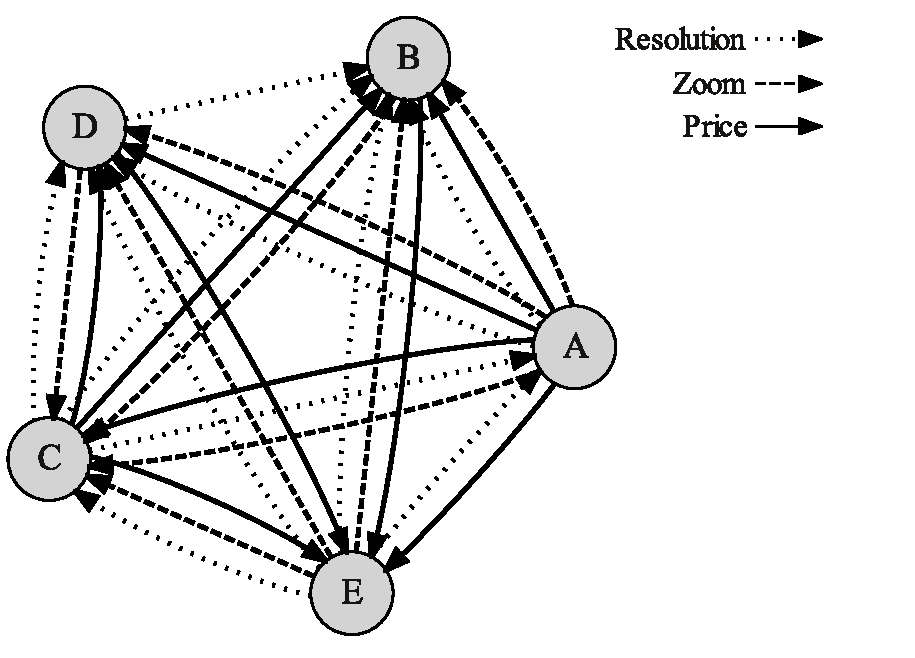
\includegraphics[width=10cm]{graphics/ProductDominationGraph}
 	\end{center}
\end{figure}

Let us give an example. We assume a choice scenario with five different cameras (see Table \ref{tab:cameras}). Product attributes are photo resolution $ph$, zoom factor $zf$, and price $pr$. All consumers have the same preference for the attribute level order: they prefer lower to higher prices, and higher photo resolutions and zoom factors to lower ones. Table \ref{tab:cameras} lists the five exemplary cameras with their corresponding attribute levels as well as single-attribute values $v_{i}$ for each attribute $a_i\in\{ph, zf, pr\}$.
Camera $E$ has the best price, but the worst photo resolution. In the product domination graph, $E$ has hence no outgoing edges with respect to price, but four outgoing edges with respect to photo resolution. Figure \ref{fig:productGraph} shows the resulting product domination graph.

Eine Tabelle finden Sie in Tabelle \ref{tab:cameras}.
\begin{table}%[!h]
	\caption{Example attribute levels and corresponding single-attribute values $v_i$}\label{tab:cameras}
	\begin{center}\small
		\begin{tabular}{lrrr}  		
			\hline
			Camera & Photo Resolution & Zoom Factor & Price\\
			\hline
			A & $v_{ph}(12 MP) = 0.60$ & $v_{zf}(10x) = 0.00$ & $v_{pr}(610 EUR) = 0.00$\\
			B & $v_{ph}(14 MP) = 1.00$ & $v_{zf}(15x) = 0.63$ & $v_{pr}(470 EUR) = 0.40$\\
			C & $v_{ph}(10 MP) = 0.20$ & $v_{zf}(18x) = 1.00$ & $v_{pr}(540 EUR) = 0.20$\\
			D & $v_{ph}(13 MP) = 0.80$ & $v_{zf}(15x) = 0.63$ & $v_{pr}(470 EUR) = 0.40$\\
			E & $v_{ph}(9 MP) = 0.00$ & $v_{zf}(10x) = 0.00$ & $v_{pr}(260 EUR) = 1.00$\\
			\hline
		\end{tabular}
	\end{center}
\end{table} 	


%
%%!TEX root = ../master.tex
\chapter{Combinatorial Auctions}
\label{chap:combinatorialAuctions}

Die ist der Ausschnitt eines Beispielkapitels.

\emph{Combinatorial auctions} (CAs) are a part of electronic
market design. Research in electronic market design joins two
disciplines: economics and computer science. Economical research
focuses on game theoretical aspects by analyzing strategic
behavior of self-interested agents. From the viewpoint of computer
science, computational problems are addressed, such as finding the
optimal allocation in auctions. As this work concentrates on
computational aspects, we assume that the reader has a stronger
background in computer science than in economics. Thus, in this
chapter we will point out the main ideas of the economical
perspective to provide some basic knowledge in this area.

\section{Mechanism Design}
\subsection{Definition}
Mechanism design was introduced by \textcite{Hu60}. It
aims at implementing system-wide solutions to problems in
non-cooperative environments with multiple self-interested agents.
Such problems can be political elections, public projects in which
the participants themselves have to invest money, or allocation
problems. Given that agents hold only private information about
their preferences, a structure has to be chosen in which in
equilibrium each agent behaves according to the designer's or principal's
intentions. The designer can either act on behalf of the society, for
example when collecting taxes for a public project, or she can
pursue self-interests when, for instance, being an auctioneer.

Since the agents' information is private, the principal faces the
problem that the agents might lie about their real valuations in
order to influence the outcome according to their preferences. In
most cases, whenever such manipulations occur, they damage the
resulting system-wide welfare \parencite{NiRo00}. Thus, simply asking
the participants to reveal their preferences is unfavorable.
Therefore, the principal has to define other rules which lead to
the desired outcome. The most common solution to this problem is
to introduce monetary transfers providing incentives for the
agents to behave truthfully.

In mechanism design two economic areas are joined: \emph{game
theory} and \emph{social choice theory}. In game theory the
agents' strategies are analyzed, and in social choice theory an
outcome is selected according to a set of agents' preferences. The
outcome in social choice theory is determined by a social choice
function, which is to be implemented by a mechanism. Formally we
have a set of possible outcomes $O$ and agents $i \in I$, $|I|=n$.
Each agent $i$ has a type $\theta_i \in \Theta_i$ reflecting the
possible preference sequences the agent can have. The type captures
all of the agent's private information relevant to her decision.
The agent's utility $u_i(o,\theta_i)$ over each outcome depends on
her type; while $u_i(o_1,\theta_i)>u_i(o_2,\theta_i)$ means that
the outcome $o_1$ is preferred over the outcome $o_2$. The social
choice function maps from the space of all types $\Theta$ to the
space of all outcomes $O$,
\begin{eqnarray}
% \nonumber to remove numbering (before each equation)
  f:\Theta_1 \times\Theta_2\times...\times\Theta_n\rightarrow O.
\end{eqnarray}
Examples for such social choice functions are allocation problems or political voting
protocols in which a candidate or a party is chosen. The most common objective of a social choice function is
the maximization of the social welfare, the so called
\emph{allocative-efficiency} \parencite{Pa01}. It maximizes the sum of
all utilities over all agents:
\begin{eqnarray}
\label{Efficient}
% \nonumber to remove numbering (before each equation)
  f(\theta)=\argmax_{o \in O} \sum_{i \in I} u_i(o,\theta_i).
\end{eqnarray}
Another objective is \emph{individual rationality}; the agent's
payoff is never less when participating in the mechanism than her
payoff without participating. Additionally there is \emph{Pareto
optimality}. An outcome is Pareto optimal whenever none of the
agents could perform better without causing another agent to
perform worse than in the current situation.

So far, we have learned what a social choice function is, and what
typical objectives for the choices of outcomes are. Now, a
mechanism has to be found which implements a given social choice
function with one or several of these objectives. For this
purpose, the agents' possible strategies have to be specified
together with an outcome function based on these strategies. The
mechanism should guarantee an implementation despite the
self-interest of the agents \parencite{Pa01}. Mathematically, a
mechanism $M$ is defined on the strategy spaces $S_i$ of the
agents:
\begin{equation}\label{MechanismDefinition}
  M=((S_1,...S_n),g(\cdot))\\
  g:S_1\times...\times S_n\rightarrow O,
\end{equation}
where $g$ is an outcome function and $S_i$ denotes all strategies
or actions an agent $i$ is allowed to take. A mechanism implements
a social choice function if there is an equilibrium strategy
profile $s^\ast(\cdot)=(s^\ast_1(\cdot),...,s^\ast_n(\cdot))$ of
the game induced by $M$ so that
\begin{equation}\label{MechanismImplements}
    g(s^\ast_1(\theta_1),...,s^\ast_n(\theta_n))=f(\theta_1,...,\theta_n),
      \quad \forall
      (\theta_1,...,\theta_n)\in(\Theta_1,...,\Theta_n),
\end{equation}
where $s^\ast_i(\theta_i)$ is the strategy agent $i$ with type
$\theta_i$ plays in the equilibrium. Please note that the
equilibrium concept is not specified in this definition. It could,
for example, be a Nash equilibrium. In this case, given the other
players $j,$ $j \neq i$, conform to the equilibrium strategies
$s^\ast_j(\theta_j)$, no other player $i$ has an incentive to
unilaterally deviate from her equilibrium strategy. Other examples
are the dominant strategy or the Bayes-Nash strategy equilibrium.
The dominant strategy equilibrium facilitates it for the agents
since the optimal strategy for an agent is independent of any
strategies the other agents could play. Thus, the agents do not
need to speculate about the way the others might behave. Informally,
we could say that the concept of dominant strategies "removes game
theory from the problem" \textcite[p.~5]{Pa01}. The Bayes-Nash
equilibrium is similar to Nash equilibriums, but assumes that
agents have incomplete information about the opponents' types.
Therefore, agents use probability functions to speculate about the
other agents' preferences \parencite{OsRu94}.

\subsection{Revelation Principle and Gibbard-Satterthwaite Theorem}
In equation \ref{MechanismDefinition}, we see that a mechanism
defines the available strategies and the function for selecting an
outcome. It is necessary that these strategies are kept simple so
that they can be applied by the agents. The easiest strategies
occur when choosing a \emph{direct mechanism} asking the agents to
report their types directly to the principal, $S_i=\Theta_i$.
Direct mechanisms lead to a centralization of the problem as
agents report their types to a center that determines the outcome
and reports it back to the agents. On the contrary, when applying
\emph{indirect mechanisms} agents have to think about how to
transform their type into a strategy and the latter is reported to
the mechanism. In other words,
\begin{quote} "the computations that go on within the mind of any
bidder in the non-direct mechanism are shifted to become part of
the mechanism in the direct mechanism". \textcite[p.~712]{McMc87}
\end{quote}
When applying these direct mechanisms agents may still lie about
their true types. Mechanisms which, in contrast, succeed in
establishing an equilibrium in which all agents tell the truth,
are called \emph{incentive-compatible}. In this case, it is in the
interest of all agents to report their true types,
$s^\ast_i(\theta_i) = \theta_i,~\forall \theta_i \in \Theta_i$.
Further, if telling the truth is a dominant strategy, the
mechanism is called \emph{strategy-proof}. As will be shown later
on, this can be achieved by the \emph{Vickrey-Clarke-Grooves}
(VCG) mechanism.

We learned that the equilibrium strategy profile $s^\ast(\cdot)$
does not determine the concept of equilibrium. Some equilibrium
concept must be chosen and implemented together with the mechanism. In the
worst case, in order to find out if a certain social choice
function can be implemented by a certain mechanism with, for
instance, dominant strategies, one would have to consider all
possible mechanisms. However, research on mechanism design led to
the \emph{revelation principle} as a solution to this. It states
that for any mechanism, there is a direct, incentive-compatible
mechanism with the same outcome \parencite{McMc87}. An intuitive
explanation for this principle consists in: the transformation
from types into strategies, which occurs in the agents' minds in
indirect mechanisms, and which is used as a filter in the direct mechanism.
That is, the direct mechanism first filters all reports of the
agents and simulates the indirect mechanism with the filtered
input. This principle is valid for the optimal mechanism as well.
Thus, the search for a mechanism can focus on direct
mechanisms. Therefore, if no direct mechanism can implement a
given social choice function, then no indirect mechanism will do
so.

In contrast to the positive result of the revelation principle,
there also exists a negative result, the
\emph{Gibbard-Satterthwaite} theorem. According to it, it is
impossible to find a mechanism with certain positive
characteristics. To understand the theorem, first note that a
social choice function is \emph{truthfully implementable} if and
only if the dominant strategy is to reveal the truth. Furthermore,
a social choice function $f$ is \emph{onto} if for each $o \in O$
at least one element in $\Theta$ exists so that $f$ maps to $o$.
Finally, a social choice function $f$ is \emph{dictatorial}
whenever there is a dictator $j$ among the agents so that for all
outcomes, $o_j$ is strictly preferred to another outcome $o_k$
whenever the dictator $j$ strictly prefers $o_j$ to $o_k$.
Obviously, this is an unwanted characteristic. It turns the
Gibbard-Satterthwaite theorem impractical for real-life mechanisms
since they allow manipulation.

\textbf{Gibbard-Satterthwaite Theorem:} \emph{Given $O$ is finite,
$|O|\geq 3$, and the social choice function $f$ is onto, then $f$
is truthfully implementable in dominant strategies if and only if
f is dictatorial}.

According to the theorem it is impossible to elicit the truth if
dominant strategies exist. However, despite this result, the
theorem can be circumvented by placing restrictions on the agents'
preferences, the way it is done in the VCG mechanism.

\subsection{Vickrey-Clarke-Grooves Mechanism}
The VCG mechanism combines the following important virtues by
introducing a special payment scheme. First, it implements social
choice functions in dominant strategies. Thus, agents do not have
to speculate which strategies the other agents might play, and
they do not need to waste resources on learning about their
competitors' strategies. Second, the mechanism does not have to
make any assumptions about the information agents have on each
other. And, third, the VCG mechanism is allocative-efficient (see
equation \ref{Efficient}), strategy-proof and non-dictatorial.

AND SO ON... 
%
%\chapter{Conclusions}\label{chap:conclusions}

Auf Deutsch: Fazit

\section{Summary}

Auf Deutsch: Zusammenfassung 

Die Zusammenfassung der Arbeit ist optional. Sollten Sie die Arbeit noch einmal zusammenfassen wollen, so halten Sie dies bitte eher kurz und wiederholen Sie sich nicht zu sehr.

\section{Limitations and Future Research}

Auf Deutsch: Limitationen und Ausblick

Es ist sinnvoll, jede Limitation an eine Idee zu knüpfen, wie diese in zukünftigen Arbeit zu adressieren waere.

\section{Contribution}

Auf Deutsch: Beitraege

Was sind die Beitraege Ihrer Arbeit sowohl für die Wissenschaft (und Theorie) als auch für die Praxis? Hier sollten Sie versuchen über den Tellerrand hinauszuschauen und einen eher weiten Blick einnehmen.





%
%\stopwordcount                         % stopwordcount
%\dumpwordcount                         % Cretaes log file
%\prettyresult                          % Gibt im Fließtext Anzahl Wörter /Seiten aus --> Auskommentieren für die Abgabe!
% ------------------------------------------------------------------------
% Hauptarbeit ENDE
% ------------------------------------------------------------------------

% ------------------------------------------------------------------------
% Erstellen des Literaturverzeichnisses
% ------------------------------------------------------------------------
\printbibliography[heading=bibintoc]  
% ------------------------------------------------------------------------
% Einbinden des Anhangs
% ------------------------------------------------------------------------
\pagenumbering{Roman}
\setcounter{page}{6}                  % ggfs. anpassen wenn Inhaltsverzeichnis länger als eine Seite

\appendix                              % Kapitel werden ab hier Alphabetisch aufgenommen
%!TEX root = ../master.tex
\chapter{Appendix}\label{Appendix}

\begin{table}[h]
\centering
\caption{Size of the search space for BASIC strategies ($n=4$).}
\label{tab:sizeSearchSpace}
 \begin{tabular}{r|r|r}
      m&s&search space size\\
      \hline
      4&1&64\\
      &2&4096\\
      &3&262,144\\
      &4&16,777,216\\
      &5&1,073,741,824\\
      7&1&262144\\
      &2&16777216\\
      &3&68,719,476,736\\
      &4&2.81E+14\\
      &5&1.15E+18\\
\end{tabular}
\end{table}



% ------------------------------------------------------------------------
% Einbinden der Eidesstaatlichen Erklärung
% ------------------------------------------------------------------------
\backmatter                            % Ab hier wird nichts mehr ins Inhaltsverzeichnis aufgenommen
%!TEX root = ../master.tex
\section*{Selbstständigkeitserklärung}
\thispagestyle{empty}
Hiermit versichere ich, die vorgelegte Thesis selbstständig und ohne unerlaubte fremde Hilfe und nur mit den Hilfen angefertigt zu haben, die ich in der Seminararbeit angegeben habe. Alle Textstellen, die wörtlich oder sinngemäß aus veröffentlichten Schriften entnommen sind, und alle Angaben die auf mündlichen Auskünften beruhen, sind als solche kenntlich gemacht. Bei den von mir durchgeführten und in der Thesis erwähnten Untersuchungen habe ich die Grundsätze guter wissenschaftlicher Praxis, wie sie in der \glqq Satzung der Justus-Liebig-Universität zur Sicherung guter wissenschaftlicher Praxisext\grqq{} niedergelegt sind, eingehalten. Gemäß \S 25 Abs. 6 der Allgemeinen Bestimmungen für modularisierte Studiengänge dulde ich eine Überprüfung der Thesis mittels Anti-Plagiatssoftware.
\bigskip

\raggedright{Gießen, den DD.MM.YYYY} \bigskip \bigskip \bigskip

Ihr NAME

\end{document}
% ----------------------------------------------------------
% Ende
% ----------------------------------------------------------
